\documentclass{article}

% Language setting
% Replace `english' with e.g. `spanish' to change the document language
\usepackage[english]{babel}
\usepackage{amsmath,amssymb}
% Set page size and margins
% Replace `letterpaper' with `a4paper' for UK/EU standard size
\usepackage[letterpaper,top=2cm,bottom=2cm,left=3cm,right=3cm,marginparwidth=1.75cm]{geometry}
\usepackage{graphicx}
\usepackage{subcaption}
\usepackage{float}
\usepackage[colorlinks=true, allcolors=blue]{hyperref}
\usepackage{adjustbox}
% Diagram
\usepackage{tikz}
\usetikzlibrary{arrows.meta,positioning,shapes.geometric}

\usepackage[section]{placeins}

\providecommand{\keywords}[1]
{
  \small	
  \textbf{\textit{Keywords---}} #1
}

\title
{Three-Stage Bearing Health Classification Using Vibration STFT and Temperature Trends in a Run-to-Failure Setting}
\author{Long Truong, Nguyen Phu Nguyen}

\begin{document}
\maketitle

\begin{abstract}
Condition-based maintenance (CBM) for rotating machinery requires not only detecting faults but also recognizing early degradation to enable timely intervention. This paper studies three-stage bearing health classification (Healthy, Degrading, Fault) using a run-to-failure dataset with two-axis vibration and temperature measurements \cite{jung2024dib_rtf,jung2024mendeley_rtf}. To better reflect deployment and avoid overly optimistic estimates caused by temporal correlation, we adopt a \textbf{leakage-aware evaluation} aligned with the time-to-failure (TTF) axis, where training samples come from earlier life segments and testing samples come from later segments. This protocol explicitly mitigates the well-known leakage from \emph{overlapped windows} when random/window-level splits are used.

Our approach converts vibration windows into time--frequency representations using short-time Fourier transform (STFT) and learns discriminative patterns with a lightweight 2D CNN. In parallel, temperature channels are summarized into compact trend/statistical descriptors and fused with vibration features via a late-fusion classifier. We report macro-averaged F1 and per-class precision/recall to account for class imbalance across life stages and compute temporal metrics over \emph{present classes} for late-life slices. In a development (file-wise stratified) setting, the model reaches Macro-F1 $\approx$ \textbf{0.7762} with per-class F1 of Healthy $\approx$ \textbf{0.69}, Degrading $\approx$ \textbf{0.64}, and Fault = \textbf{1.00}. 
In a leakage-aware temporal evaluation focused on late-life behavior where only Degrading/Fault are present, the model achieves Accuracy $\approx$ \textbf{0.95} and Macro-F1 $\approx$ \textbf{0.9467} over the present classes. Our study is a \emph{proof of concept} on a single run; we highlight the evaluation protocol and multi-modal fusion as practical choices for realistic deployment and outline validation on additional datasets as future work.
\end{abstract}
\keywords{bearing health monitoring,run-to-failure, degradation stage classification, STFT spectrogram, vibration–temperature fusion, temporal split, condition-based maintenance.}

\section{Introduction}
\label{sec:intro}

Rotating machinery is a core asset in modern industry, and rolling-element bearings are among the most failure-prone components due to continuous mechanical stress, friction, and thermal loading. Unexpected bearing failures can cause unplanned downtime, safety risks, and substantial maintenance costs. Consequently, \emph{condition-based maintenance} (CBM) and \emph{prognostics and health management} (PHM) aim to continuously monitor bearing health and trigger maintenance actions before critical breakdowns.

Vibration-based diagnosis has been widely explored, where deep learning models---especially convolutional neural networks (CNNs)---learn discriminative patterns from raw waveforms or time--frequency representations such as spectrograms. However, practical CBM deployment often needs more than binary ``healthy vs.\ fault'' decisions. In run-to-failure monitoring, an intermediate \emph{degrading} stage is crucial for early warning, but it is also the hardest to recognize due to subtle signal changes, class imbalance, and evolving operating conditions \cite{jung2024dib_rtf}.

A second challenge is \emph{evaluation realism}. Many bearing diagnostic studies rely on random or window-level splits that inadvertently leak temporally adjacent samples across train/test, yielding overly optimistic performance \cite{wheat2024leakage,vieira2024realistic}. In real deployments, models must generalize from earlier-life behavior to later-life degradation patterns that were not observed during training. Therefore, leakage-aware temporal protocols aligned with the time-to-failure (TTF) axis are necessary to estimate true field performance.

Finally, multi-sensor information can improve stage recognition. Temperature is often correlated with friction and abnormal thermal behavior, providing complementary evidence to vibration signals, especially near degradation onset \cite{huang2023esrel_tempvib}. Yet effectively fusing temperature with vibration while keeping the model lightweight remains non-trivial.

In this work, we address three-stage bearing health classification (Healthy, Degrading, Fault) under a run-to-failure setting using vibration STFT representations and temperature trend descriptors \cite{jung2024dib_rtf,jung2024mendeley_rtf}. The key idea is to couple (i) time--frequency CNN features from vibration with (ii) compact temperature trend/statistical descriptors via a late-fusion classifier, and (iii) validate performance using leakage-aware temporal splits aligned with TTF.
To bridge development and deployment, we follow a two-phase workflow: we first train a baseline model under a file-wise stratified split, and then perform leakage-aware temporal fine-tuning aligned with the TTF axis (train [0,60]\%, val [60,70]\%, test [70,100.1]\%). This design explicitly tests generalization from earlier-life behavior to later-life degradation while reducing the optimistic bias caused by temporally overlapped windows.
\textbf{Contributions.} This paper makes the following contributions:
\begin{itemize}
    \item We formulate a three-stage bearing health classification problem on a run-to-failure dataset with synchronized two-axis vibration and temperature measurements \cite{jung2024dib_rtf,jung2024mendeley_rtf}.
    \item This two-phase scheme (stratified pre-training $\rightarrow$ temporal fine-tuning) provides a clearer separation between development validation and deployment-oriented testing, preventing temporal leakage across overlapping windows.
    \item We adopt and emphasize a leakage-aware evaluation protocol aligned with the TTF timeline, which better matches deployment and mitigates optimistic bias from temporal leakage \cite{wheat2024leakage,vieira2024realistic}.
\end{itemize}

\section{Related Work}
\label{sec:related_work}

\subsection{Bearing fault diagnosis with deep learning and time--frequency representations}
Deep learning has become a dominant approach for rolling-element bearing diagnosis due to its ability to learn discriminative patterns directly from sensor signals. A common pipeline transforms vibration windows into 2D time--frequency images (e.g., STFT spectrograms or wavelet scalograms) and applies 2D CNNs originally developed for vision tasks. Verstraete et al.~\cite{verstraete2017tf} demonstrated that time--frequency image analysis combined with CNNs can achieve strong fault diagnosis performance and influenced subsequent spectrogram/scalogram-based methods.
More recent studies continue to explore CNN architectures and feature learning strategies for robust vibration-based fault recognition \cite{magar2020faultnet}.

While these methods are effective for identifying explicit fault signatures, run-to-failure monitoring often requires recognizing an intermediate degradation stage in addition to the final fault stage. This setting introduces higher ambiguity and stronger class imbalance, making Degrading detection more challenging than binary fault classification.

We adapt parts of an open-source CNN implementation for bearing diagnosis~\cite{mdzalfirdausi_paderborn_repo}, and extend it with temperature fusion, STFT normalization tailored to run-to-failure windows, and leakage-aware TTF-aligned evaluation.
\subsection{Run-to-failure data and degradation-stage recognition}
Run-to-failure datasets provide realistic progression of health states but also raise challenges in label definition and evaluation. The bearing run-to-failure dataset used in this work includes vibration and temperature streams over the asset lifetime \cite{jung2024dib_rtf,jung2024mendeley_rtf}. Prior studies on run-to-failure monitoring frequently rely on stage labels derived from time or degradation indicators, aiming to approximate early-life, mid-life, and late-life behaviors. However, the intermediate stage is often under-represented and may overlap with healthy behavior, which motivates integrating complementary sensing modalities and carefully designing evaluation protocols.
\paragraph{Stage-based monitoring vs. RUL prognostics.}
Beyond fault recognition, PHM research often targets remaining useful life (RUL) estimation using regression or sequence models. However, reliable RUL supervision and consistent degradation indicators are not always available in practical run-to-failure experiments. As an alternative, stage-based health classification provides actionable early-warning signals with weaker supervision, which aligns with many CBM decision processes. In this work, we focus on three-stage health recognition to support timely maintenance actions under realistic labeling constraints.
\subsection{Evaluation protocols and data leakage in bearing diagnostics}
A growing body of work highlights that random splitting of highly overlapped windows can cause severe information leakage: temporally adjacent windows share similar spectral content, and if they appear in both training and testing, performance can be inflated \cite{wheat2024leakage}. Vieira et al.~\cite{vieira2024realistic} further argue for more realistic evaluation strategies in machine diagnostics that reflect the operational reality of future data being unseen at training time. These findings motivate leakage-aware temporal splits aligned with the time-to-failure axis, which we adopt as a primary evaluation protocol to better approximate deployment performance.
In addition to temporal leakage, generalization across different bearings or operating conditions (domain shift) remains challenging in machine diagnostics. While fully bearing-wise evaluation may require larger cross-unit coverage, our TTF-aligned temporal protocol is a necessary first step toward deployment realism by preventing near-duplicate windows from leaking across splits.
\subsection{Multi-sensor fusion with temperature and vibration}
Multi-sensor learning is a practical direction for improving robustness, as temperature may capture thermal effects associated with friction, lubrication issues, or abnormal contact conditions. Huang et al.~\cite{huang2023esrel_tempvib} showed that combining temperature-related signals with vibration features can improve diagnostic performance compared with single-sensor baselines. Inspired by this direction, we fuse vibration time--frequency CNN features with compact temperature trend/statistical descriptors, aiming to improve Degrading-stage recognition in run-to-failure monitoring while keeping the model lightweight.

\section{Methodology}
\label{sec:method}

\subsection{Overview}
We propose a lightweight multi-modal pipeline for bearing health stage recognition. For each 1.0-s window, we transform two-axis vibration into a 2-channel log-spectrogram image and summarize two-channel temperature into a compact 6-D descriptor. A small ResNet-style CNN encodes vibration patterns, a linear layer embeds temperature features, and a late-fusion classifier predicts the health stage. To bridge development and deployment, we adopt a two-phase workflow: stratified training followed by leakage-aware temporal fine-tuning along the TTF axis. Implementation-wise, our code adapts components from an open-source repository~\cite{mdzalfirdausi_paderborn_repo} and customizes them for TTF-aligned temporal splitting, per-window/per-frequency spectrogram normalization, temperature-fusion at the head, and file-wise mean-logit aggregation.

\subsection{Block Diagram}
Figure~\ref{fig:block} illustrates the end-to-end data flow from raw inputs to file-wise decisions and where fusion occurs.

\begin{figure}[H]
  \centering
  \begin{adjustbox}{max width=\linewidth}
  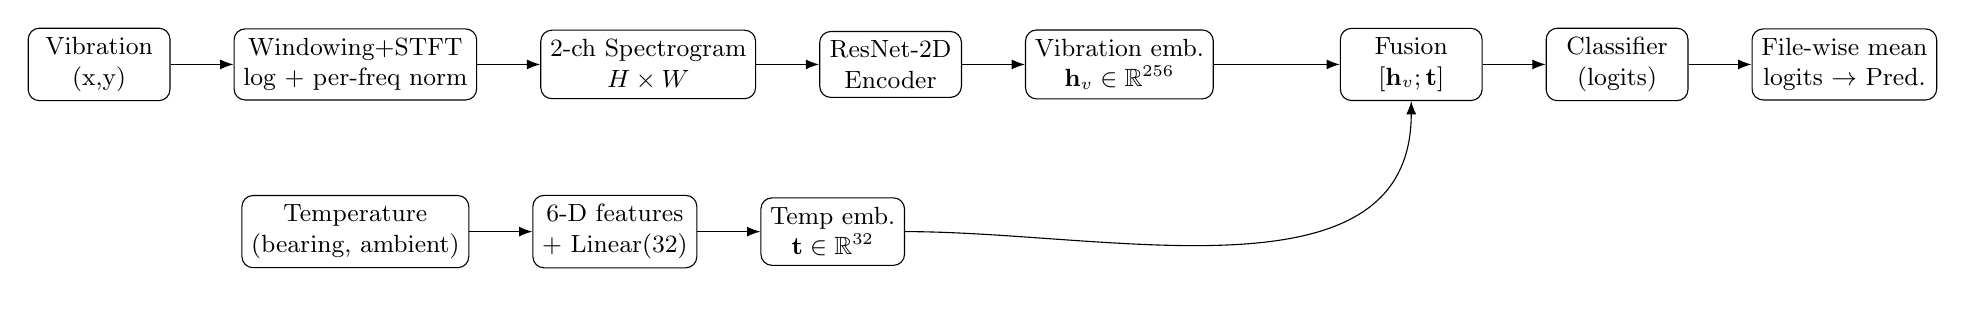
\begin{tikzpicture}[
    node distance=8mm and 8mm,
    box/.style={draw, rounded corners, align=center, minimum height=7mm, minimum width=18mm, font=\small},
    arr/.style={-Latex}
  ]
    % Top chain (compact)
    \node[box] (vib) {Vibration\\(x,y)};
    \node[box, right=of vib] (wstft) {Windowing+STFT\\log + per-freq norm};
    \node[box, right=of wstft] (spec) {2-ch Spectrogram\\$H\times W$};
    \node[box, right=of spec] (cnn) {ResNet-2D\\Encoder};
    \node[box, right=of cnn] (vz) {Vibration emb.\\$\mathbf{h}_v\in\mathbb{R}^{256}$};

    % Temp branch (compact)
    \node[box, below=12mm of wstft, xshift=0mm] (temp) {Temperature\\(bearing, ambient)};
    \node[box, right=of temp] (tfeat) {6-D features\\+ Linear(32)};
    \node[box, right=of tfeat] (tz) {Temp emb.\\$\mathbf{t}\in\mathbb{R}^{32}$};

    % Fusion + classifier + aggregation
    \node[box, right=16mm of vz] (fuse) {Fusion\\$[\mathbf{h}_v;\mathbf{t}]$};
    \node[box, right=of fuse] (cls) {Classifier\\(logits)};
    \node[box, right=of cls] (agg) {File-wise mean\\logits $\to$ Pred.};

    % Arrows top chain
    \draw[arr] (vib) -- (wstft);
    \draw[arr] (wstft) -- (spec);
    \draw[arr] (spec) -- (cnn);
    \draw[arr] (cnn) -- (vz);

    % Temp arrows
    \draw[arr] (temp) -- (tfeat);
    \draw[arr] (tfeat) -- (tz);

    % Fusion arrows
    \draw[arr] (vz) -- (fuse);
    % Route temp embedding to fusion from below to avoid crossing blocks
    \draw[arr] (tz.east) to[out=0,in=270] (fuse.south);
    \draw[arr] (fuse) -- (cls);
    \draw[arr] (cls) -- (agg);
  \end{tikzpicture}
  \end{adjustbox}
  \caption{Block diagram of the proposed multi-modal pipeline with late fusion and file-wise mean-logit aggregation.}
  \label{fig:block}
\end{figure}

\subsection{Synchronous windowing for vibration and temperature}
In the current codebase, vibration and temperature are sampled synchronously at 25.6 kHz and stored as four channels per sample (two vibration axes + two temperature channels). We segment the raw sequence into 1.0-s windows with 50\% overlap (hop 0.5 s). For each window with indices $[s:e]$, we slice vibration and temperature using the same indices:
$\mathbf{x}_v=\mathrm{arr}[s:e,0{:}2]$ and $\mathbf{x}_t=\mathrm{arr}[s:e,2{:}4]$.
This design avoids any additional timestamp alignment. If temperature were sampled at a different rate, an explicit resampling/alignment step would be required.

\subsection{Waveform sanitization and per-window z-score}
Before computing time--frequency features, we sanitize each vibration window by replacing NaN/Inf values with zeros. Then we apply per-window, per-channel z-score normalization:
\begin{equation}
\mathbf{x}'_{v,k} = \frac{\mathbf{x}_{v,k} - \mu(\mathbf{x}_{v,k})}{\sigma(\mathbf{x}_{v,k})+\epsilon},\quad k\in\{1,2\},
\end{equation}
where $\mu(\cdot)$ and $\sigma(\cdot)$ are computed within the 1.0-s window for each axis, and $\epsilon$ is a small constant for numerical stability.

\subsection{STFT magnitude and log-compression}
Each vibration window is converted to a time--frequency representation using STFT with $n\_{fft}=4096$, $hop\_length=1024$, and a Hann window. The magnitude is log-compressed and normalized as described in Section~\ref{sec:method}, then resized to a fixed $224\times224$ resolution.
We take magnitude and apply log-compression to reduce dynamic range:
\begin{equation}
\mathbf{S}_k = \log\left(1 + \alpha |\mathbf{X}_k|\right),
\end{equation}
where $\alpha=1.0$ (i.e., \texttt{torch.log1p(mag * log\_add)} with \texttt{log\_add=1.0}).

\subsection{Per-frequency normalization across time frames}
To stabilize ``brightness'' variations across frames, we normalize each frequency bin across the time dimension (z-score over frames for each frequency):
\begin{equation}
\tilde{\mathbf{S}}_k(f,t)=\frac{\mathbf{S}_k(f,t)-\mu_t(\mathbf{S}_k(f,\cdot))}{\sigma_t(\mathbf{S}_k(f,\cdot))+\epsilon}.
\end{equation}
This step is performed independently for each vibration axis.

\subsection{Resize and channel stacking}
We resize each normalized spectrogram $\tilde{\mathbf{S}}_k$ to the target size $H\times W$ (current configuration: $224\times224$) using bilinear interpolation. The two axes are then stacked as channels:
\begin{equation}
\mathbf{S}=\mathrm{stack}(\tilde{\mathbf{S}}_1,\tilde{\mathbf{S}}_2)\in\mathbb{R}^{2\times H \times W},
\end{equation}
forming the CNN input for each window.

\subsection{Temperature descriptor (6-D) per window}
From the two temperature channels (bearing and ambient) sliced by the same indices $[s:e]$, we compute a 6-D descriptor:
\begin{equation}
\mathbf{h}_t = [\mu_b, \sigma_b, s_b, \mu_a, \sigma_a, s_a]\in\mathbb{R}^{6},
\end{equation}
where $\mu$ and $\sigma$ are mean and standard deviation within the 1.0-s window, and $s$ is the least-squares slope over the sample index within the window. Non-finite values are ignored; if a channel contains no finite values, its three descriptors are set to zero.

\subsection{Vibration encoder: lightweight ResNet-18 variant}
We encode spectrogram inputs with a compact ResNet-18-style 2D CNN configured for two input channels. The stem uses a $7\times7$ convolution with stride 2 and 32 channels, followed by batch normalization, ReLU, and max pooling. Four stages of BasicBlocks follow with channel progression:
32$\rightarrow$32 (stride 1), 32$\rightarrow$64 (stride 2), 64$\rightarrow$128 (stride 2), and 128$\rightarrow$256 (stride 2). A global average pooling layer produces a 256-D vibration embedding $\mathbf{h}_v\in\mathbb{R}^{256}$.

\subsection{Late fusion classifier}
Temperature features are projected via a linear layer and ReLU:
\begin{equation}
\mathbf{t} = \mathrm{ReLU}(\mathbf{W}_t \mathbf{h}_t + \mathbf{b}_t)\in\mathbb{R}^{32}.
\end{equation}
We then concatenate vibration and temperature embeddings and apply a linear classifier:
\begin{equation}
\mathbf{u} = [\mathbf{h}_v;\mathbf{t}] \in \mathbb{R}^{288},\quad
\boldsymbol{\ell} = \mathbf{W}_c \mathbf{u} + \mathbf{b}_c,
\end{equation}
where $\boldsymbol{\ell}$ denotes the pre-softmax logits and $\hat{\mathbf{p}}=\mathrm{softmax}(\boldsymbol{\ell})$.
No dropout is used in the fusion head in the current configuration.

\subsection{File-wise inference via mean \emph{pre-softmax} logit aggregation}
\label{sec:filewise}

Window-level training uses mini-batches with $\mathbf{S}\in\mathbb{R}^{B\times2\times H\times W}$ and $\mathbf{h}_t\in\mathbb{R}^{B\times6}$. 
For file-wise evaluation, we forward all windows belonging to the same file and collect their \emph{pre-softmax} logit vectors $\{\boldsymbol{\ell}_i\}_{i=1}^{n}$, where $\boldsymbol{\ell}_i\in\mathbb{R}^{C}$ and $C$ is the number of classes. 
We aggregate window-level evidence by averaging logits and then predicting the file label by $\arg\max$:
\begin{equation}
\bar{\boldsymbol{\ell}} = \frac{1}{n}\sum_{i=1}^{n}\boldsymbol{\ell}_i,\quad
\hat{y}_{\text{file}}=\arg\max_{c \in \{1,\dots,C\}} \bar{\ell}_c.
\end{equation}
Averaging \emph{pre-softmax} logits (rather than probabilities) yields a simple and stable file-level decision rule and is used consistently in our evaluation pipeline.
\paragraph{Implementation provenance.}

Parts of our implementation were adapted and refactored from an open-source repository for CNN-based bearing diagnosis~\cite{mdzalfirdausi_paderborn_repo}. We substantially modified the pipeline to support run-to-failure windowing, two-axis STFT spectrogram construction with per-window and per-frequency normalization, temperature-feature fusion, and leakage-aware TTF-aligned temporal fine-tuning and evaluation.
\subsection{Two-phase training: stratified learning and temporal fine-tuning}
We train in two phases. First, we learn a baseline model using file-wise stratified splitting for development validation. Second, we perform leakage-aware temporal fine-tuning aligned with the TTF axis (train [0,60]\%, val [60,70]\%, test [70,100.1]\%). This temporal protocol mitigates optimistic bias caused by overlapped-window leakage and better reflects deployment, where future (later-life) data are unseen during training.
\paragraph{Practical temporal fine-tuning details.}
We initialize temporal fine-tuning from the best stratified checkpoint (\texttt{init\_from}). We enable balanced sampling, cap validation cost with \texttt{val\_max\_windows}=50, and fine-tune with AdamW (lr $3\times10^{-5}$, weight decay $10^{-2}$) under a cosine schedule (OneCycle disabled) with AMP enabled.
\subsection{Computational complexity and runtime}
\label{sec:complexity}

Our model is designed to be lightweight. The vibration branch uses a compact ResNet-18 variant with reduced channel widths (32--256) and global average pooling, while the temperature branch is a single linear projection (6$\rightarrow$32) followed by a linear classifier on the fused 288-D vector. Thus, the additional cost of temperature fusion is negligible compared to the CNN forward pass.

The dominant computation comes from (i) STFT feature construction and (ii) the 2D CNN encoder. STFT is computed once per 1.0-s window with fixed parameters ($n\_{fft}=4096$, $hop=1024$), and the resulting spectrogram is resized to $224\times224$. The CNN then processes a 2-channel input of size $224\times224$, yielding a 256-D embedding. File-wise inference further amortizes window-level noise by averaging logits across windows, requiring only a single pass per window and an $\mathcal{O}(nC)$ aggregation over $n$ windows and $C$ classes.

In practice, this pipeline supports efficient training with AMP and enables fast inference suitable for near-real-time monitoring, as both the fusion head and the file-wise aggregation introduce minimal overhead beyond the CNN backbone.

To reduce evaluation overhead during training and fine-tuning, we cap validation computation by limiting the number of evaluated windows per file (\texttt{val\_max\_windows}=50), which improves iteration speed without changing the inference pipeline.

\section{Dataset and Problem Definition}
\label{sec:data_problem}

\subsection{Run-to-failure dataset}
We use the run-to-failure bearing dataset provided by Jung et al.~\cite{jung2024dib_rtf,jung2024mendeley_rtf}. 
The dataset contains \textbf{one run} (\texttt{RUNS=1}) consisting of \textbf{129 files} (\texttt{FILES=129}). 
Two-axis vibration signals are sampled at \textbf{25.6 kHz}.

\subsection{Segmentation and feature construction}
We segment vibration into fixed-length windows of \textbf{1.0 s} (25{,}600 samples) with \textbf{50\% overlap} (hop = 0.5 s = 12{,}800 samples). 
Each vibration window is converted to a time--frequency representation using STFT with $n\_fft \in \{2048,4096\}$ and $hop\_length \in \{512,1024\}$. 
The resulting spectrogram is resized to \textbf{$160\times160$} for the development setting and \textbf{$224\times224$} for the temporal fine-tuning setting.

In addition, we extract temperature features from \textbf{two channels}. 
For each window, we compute \textbf{six} temperature descriptors: mean, standard deviation, and slope for each channel (total 6-D).

\subsection{Three-stage health definition by normalized lifetime}
Let $\mathrm{TTF\%} \in [0,1]$ denote the normalized time-to-failure percentage within the run. 
We define three health stages using thresholds $\tau_1$ and $\tau_2$:
\begin{equation}
y=
\begin{cases}
\text{Healthy}, & 0 \le \mathrm{TTF\%} < 0.60,\\
\text{Degrading}, & 0.60 \le \mathrm{TTF\%} < 0.90,\\
\text{Fault}, & 0.90 \le \mathrm{TTF\%} \le 1.00.
\end{cases}
\label{eq:stage_labeling}
\end{equation}
We choose $\tau_1=0.60$ and $\tau_2=0.90$ to represent early-, mid-, and late-life regions, respectively. 
These thresholds are used to design realistic temporal splits along the lifetime axis. In practice, we selected $\tau_1$ and $\tau_2$ from empirical observation of our run's label distribution and sensor trends (e.g., rising thermal load and spectral changes towards late life), which place the Degrading onset near $\sim$60\% and Fault concentration beyond $\sim$90\% TTF.

\paragraph{Physical rationale and limitations.} Although chosen empirically on this run, these cutoffs are consistent with typical bearing degradation signatures observed in vibration and temperature: around mid-life, gradual increases in broadband energy, emergent sidebands around characteristic defect frequencies (e.g., BPFI/BPFO), and a sustained upward drift in temperature often appear; near end-of-life, severe faulting produces pronounced harmonics and modulation sidebands together with higher and more volatile thermal load. We do not claim universality: the exact transition points depend on bearing design, loading, lubrication, and operating conditions. In future work, we will (i) test sensitivity to $(\tau_1,\tau_2)$, and (ii) explore physics-guided or data-driven boundaries via change-point detection on envelope spectra, RMS/kurtosis trends, or temperature slope to align thresholds more closely with underlying physical changes.

\section{Experimental Setup}
\label{sec:setup}

\subsection{Development setting: stratified split}
We first evaluate in a development setting using file-wise stratified splitting with train/val/test ratios of 0.6/0.2/0.2 and a minimum of 5 samples per class in validation and test. 
We train with AdamW (learning rate $2\times10^{-4}$, weight decay $10^{-3}$) for up to 80 epochs. 
We use label smoothing of 0.05, balanced sampling, and automatic mixed precision (AMP). 
Early stopping is applied with patience 20, selecting the best checkpoint by macro-F1.

\begin{table}[htbp]
\centering
\begin{tabular}{lcc}
\hline
 & Stratified (dev) & Temporal (FT) \\
\hline
Split & 0.6/0.2/0.2 & [0,60]/[60,70]/[70,100.1]\% \\
Init & scratch & best stratified (\texttt{init\_from}) \\
Optimizer & AdamW & AdamW \\
LR & $2\times10^{-4}$ & $3\times10^{-5}$ \\
Weight decay & $10^{-3}$ & $10^{-2}$ \\
Epochs & 80 & 60 \\
Sampling & balanced & balanced \\
Schedule & -- & cosine (OneCycle off) \\
AMP & on & on \\
Early stop & 20 & 12 \\
val\_max\_windows & -- & 50 \\
\hline
\end{tabular}
\caption{Training and evaluation settings for stratified development and temporal fine-tuning.}
\label{tab:settings}
\end{table}

\subsection{Deployment-oriented setting: leakage-aware temporal split}
These settings differ from common random-split diagnostic baselines by enforcing strict TTF-aligned temporal separation to mitigate leakage.

To reduce temporal leakage and better match deployment, we adopt a TTF-aligned temporal split: train [0,60]\%, val [60,70]\%, and test [70,100.1]\%. 
We initialize from the best stratified checkpoint (\texttt{best.pt}) and fine-tune using AdamW (learning rate $3\times10^{-5}$, weight decay $10^{-2}$) for up to 60 epochs with early stopping patience 12. 
We keep balanced sampling and AMP enabled, and use cosine scheduling (OneCycle disabled). 
To stabilize validation cost, we set \texttt{val\_max\_windows}=50.

\begin{figure}[H]
  \centering
  % Sử dụng tùy chọn [b] để căn lề dưới cho các subfigure
  \begin{subfigure}[b]{0.48\textwidth}
    \centering
    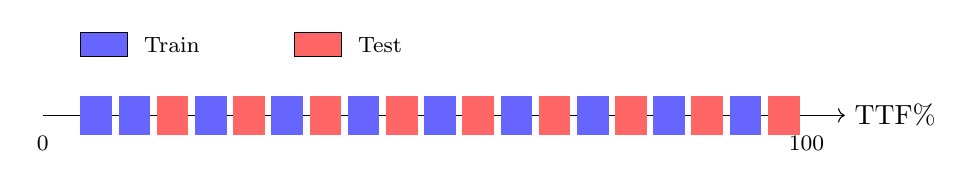
\begin{tikzpicture}[x=0.08\linewidth, y=6mm]
      % Trục TTF
      \draw[->] (0,0) -- (10.5,0) node[right]{TTF\%};
      \node at (0,-0.6){\footnotesize 0}; \node at (10,-0.6){\footnotesize 100};
      
      % Các khối cửa sổ xen kẽ (Train/Test) minh họa rủi ro rò rỉ
      \foreach \x/\c in {0.5/blue!60,1/blue!60,1.5/red!60,2/blue!60,2.5/red!60,3/blue!60,3.5/red!60,4/blue!60,4.5/red!60,5/blue!60,5.5/red!60,6/blue!60,6.5/red!60,7/blue!60,7.5/red!60,8/blue!60,8.5/red!60,9/blue!60,9.5/red!60} {
        \draw[fill=\c,draw=\c] (\x,-0.4) rectangle ++(0.4,0.8);
      }
      
      % Chú thích (Legend) - Phần này làm hình (a) cao hơn hình (b)
      \draw[fill=white, draw=white] (0.5,1.38) rectangle (3.4,1.62);
      \node[draw, fill=blue!60, minimum width=6mm, minimum height=3mm] (l1) at (0.8,1.5) {};
      \node[anchor=west] at (1.2,1.5) {\footnotesize Train};
      \node[draw, fill=red!60, minimum width=6mm, minimum height=3mm] (l2) at (3.6,1.5) {};
      \node[anchor=west] at (4,1.5) {\footnotesize Test};
    \end{tikzpicture}
    \caption{Random/window split (leakage risk).}
  \end{subfigure}
  \hfill
  \begin{subfigure}[b]{0.48\textwidth}
    \centering
    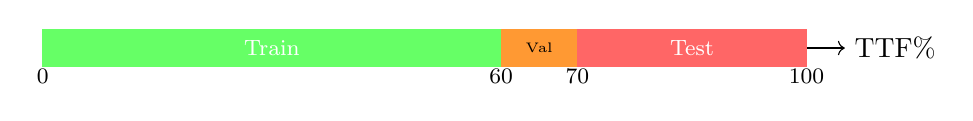
\begin{tikzpicture}[x=0.08\linewidth, y=6mm]
      % Trục TTF
      \draw[->] (0,0) -- (10.5,0) node[right]{TTF\%};
      \node at (0,-0.6){\footnotesize 0}; \node at (6,-0.6){\footnotesize 60}; \node at (7,-0.6){\footnotesize 70}; \node at (10,-0.6){\footnotesize 100};
      
      % Các khối phân chia theo dòng thời gian (Train 60%, Val 10%, Test 30%)
      \draw[fill=green!60,draw=green!60] (0,-0.4) rectangle (6,0.4);
      \node[color=white, font=\footnotesize] at (3,0) {Train};
      
      \draw[fill=orange!80,draw=orange!80] (6,-0.4) rectangle (7,0.4);
      \node[font=\tiny] at (6.5,0) {Val};
      
      \draw[fill=red!60,draw=red!60] (7,-0.4) rectangle (10,0.4);
      \node[color=white, font=\footnotesize] at (8.5,0) {Test};
    \end{tikzpicture}
    \caption{TTF-aligned temporal split (leakage-aware).}
  \end{subfigure}
  
  \caption{Protocol comparison: window-level random split interleaves overlapped windows across time (leakage) versus contiguous TTF-aligned temporal split that prevents near-duplicate windows from crossing splits.}
  \label{fig:protocol_compare}
\end{figure}



\section{Results}
\label{sec:results}

\subsection{Stratified evaluation (3-class)}
In the stratified development setting, our best configuration (\texttt{auto\_r22}) achieves \textbf{Macro-F1 = 0.7762}. 
Per-class F1 scores are approximately: Healthy $\approx$ 0.69, Degrading $\approx$ 0.64, and Fault = 1.00. 
This indicates that Fault signatures are highly separable, while the Degrading stage remains the most challenging due to its transitional nature.

Figure~\ref{fig:strat_pair} summarizes the stratified confusion matrix and per-class F1.

\begin{figure}[H]
  \centering
  \begin{subfigure}[H]{0.48\textwidth}
    \centering
    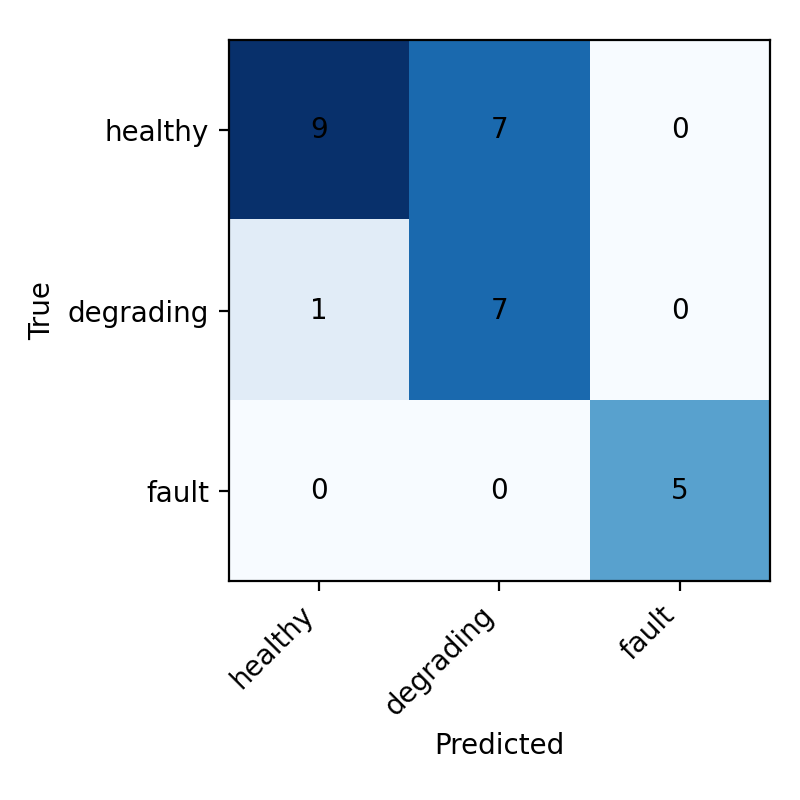
\includegraphics[width=\linewidth]{figures/stratified/confusion_matrix.png}
    \caption{Confusion matrix (stratified, 3-class).}
    \label{fig:cm_strat_sub}
  \end{subfigure}
  \hfill
  \begin{subfigure}[H]{0.48\textwidth}
    \centering
    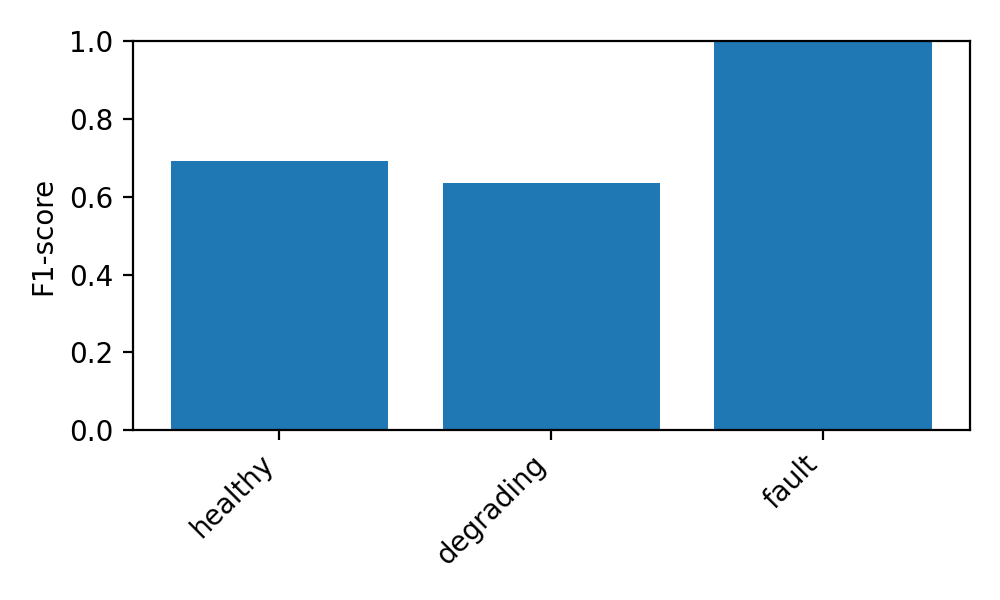
\includegraphics[width=\linewidth]{figures/stratified/f1_per_class.png}
    \caption{Per-class F1 (stratified).}
    \label{fig:f1_strat_sub}
  \end{subfigure}
  \caption{Stratified evaluation (3-class): confusion matrix and per-class F1.}
  \label{fig:strat_pair}
\end{figure}

\subsection{Temporal evaluation (deployment-oriented)}
Under the temporal leakage-aware split, the test slice [70,100.1]\% corresponds to late-life behavior where \emph{Healthy samples do not appear}. 
Therefore, we report metrics over the \emph{present classes} (Degrading and Fault). 
In this setting, the model reaches \textbf{Accuracy $\approx$ 0.95} and \textbf{Macro-F1 $\approx$ 0.9467}, with F1 scores of Degrading $\approx$ 0.9333 and Fault $\approx$ 0.9600. 
These results suggest that the learned representation transfers well from earlier life to late-life discrimination when evaluated without temporal leakage.



Figure~\ref{fig:temporal_pair} summarizes temporal performance on the late-life slice.
\begin{figure}[htbp]
  \centering
  \begin{subfigure}[htbp]{0.48\textwidth}
    \centering
    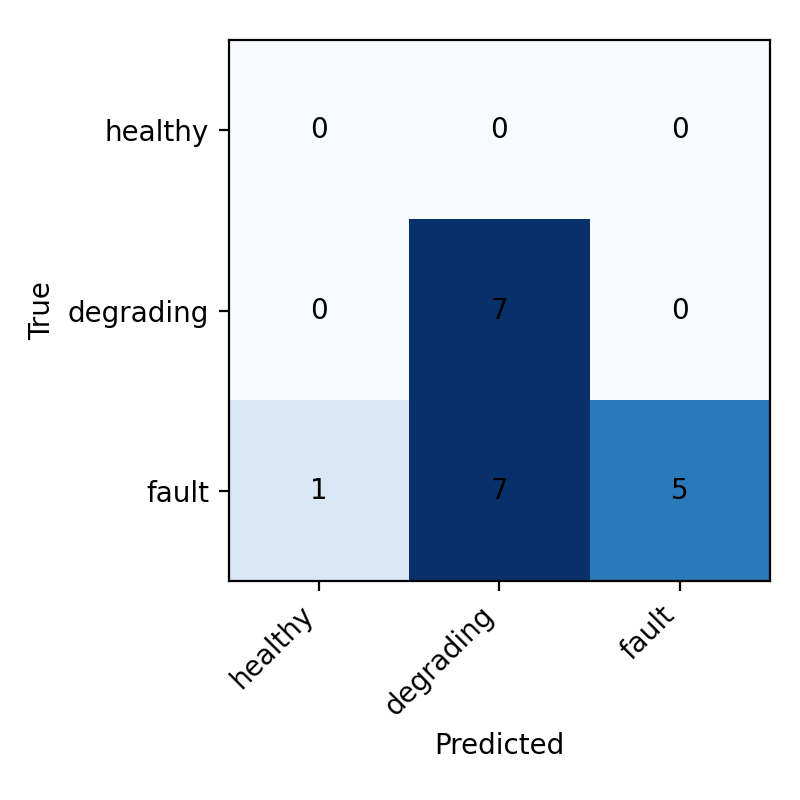
\includegraphics[width=\linewidth]{figures/temporal/confusion_matrix.png}
    \caption{Confusion matrix (temporal [70,100.1]\% TTF).}
    \label{fig:cm_temporal_sub}
  \end{subfigure}
  \hfill
  \begin{subfigure}[htbp]{0.48\textwidth}
    \centering
    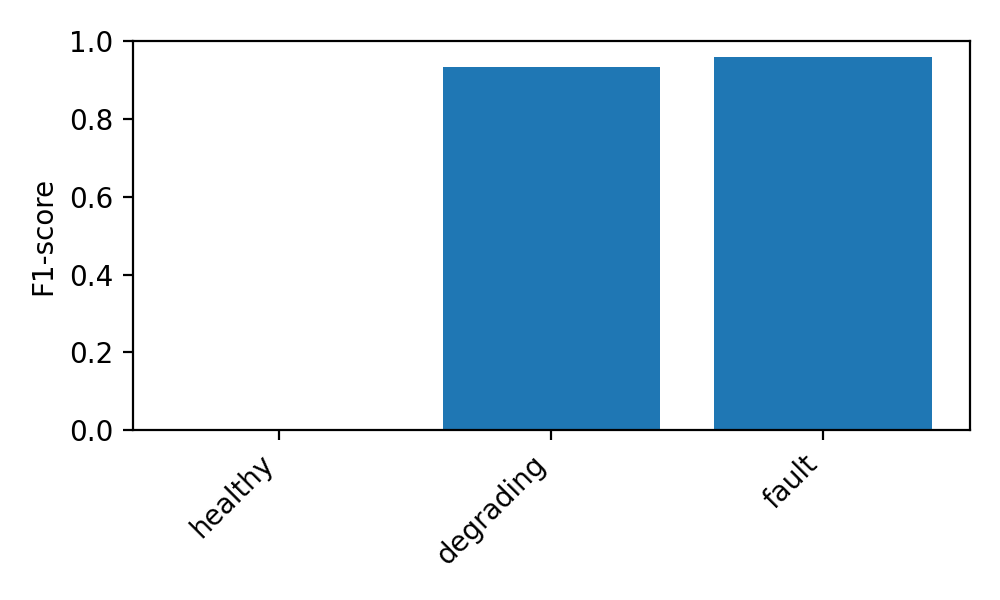
\includegraphics[width=\linewidth]{figures/temporal/f1_per_class.png}
    \caption{Per-class F1 (present classes only).}
    \label{fig:f1_temporal_sub}
  \end{subfigure}
  \caption{Leakage-aware temporal evaluation on the late-life slice [70,100.1]\% TTF, where only Degrading and Fault are present. Metrics are reported over present classes.}
  \label{fig:temporal_pair}
\end{figure}

\subsection{Failure case analysis with broader temporal coverage}
When expanding evaluation to a broader range that includes more ambiguous mid-life samples, performance drops substantially (Accuracy $\approx$ 0.3333, Macro-F1 $\approx$ 0.3324), where Degrading is frequently confused with Healthy and Healthy may have zero support depending on the slice.  
This behavior highlights that the decision boundary between Healthy and early Degrading is sensitive and requires either (i) stronger supervision/labeling for the transition region, (ii) richer temperature trend modeling, or (iii) sequence-aware modeling that leverages longer temporal context. 

\subsection{Ablation Studies}
\label{sec:ablation}

\paragraph{Effect of stratified initialization.}
We compare temporal fine-tuning initialized from the best stratified checkpoint (two-phase) against fine-tuning from scratch. On a late-life slice where Degrading and Fault are present (e.g., $[85,100.1]\%$ TTF), the two-phase model achieves strong two-class performance (present-label macro F1 $\approx 0.947$), whereas training from scratch collapses toward the dominant class on the same late coverage (present-label macro F1 $\approx 0.250$). Figure~\ref{fig:abl_init} contrasts confusion matrices.

\begin{figure}[htbp]
  \centering
  \begin{subfigure}[htbp]{0.48\textwidth}
    \centering
    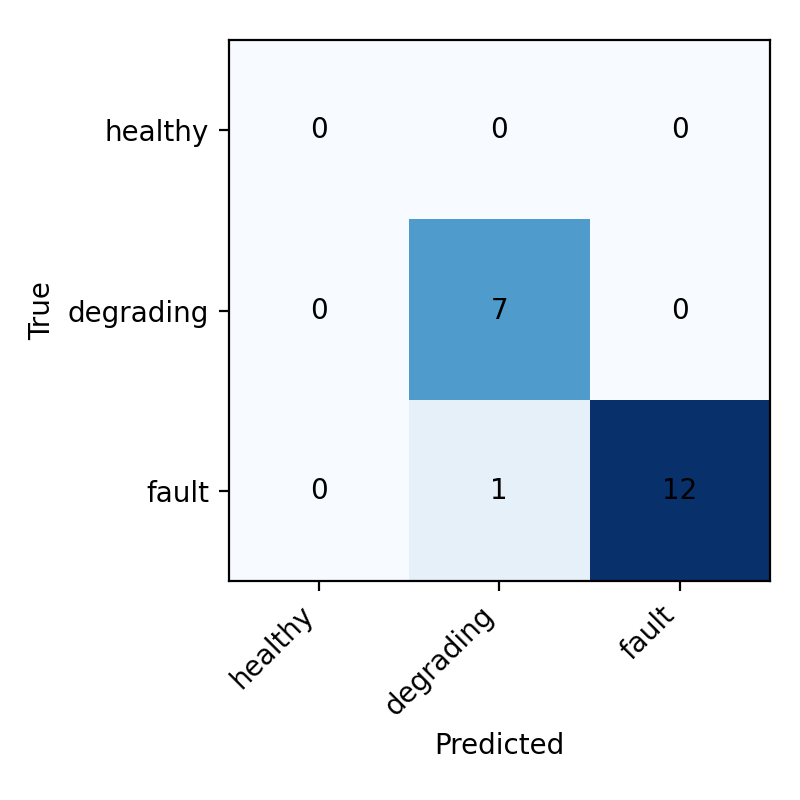
\includegraphics[width=\linewidth]{figures/ablation/temporal_ft_r2_confusion.png}
    \caption{With stratified init (late-life, two-phase).}
  \end{subfigure}
  \hfill
  \begin{subfigure}[htbp]{0.48\textwidth}
    \centering
    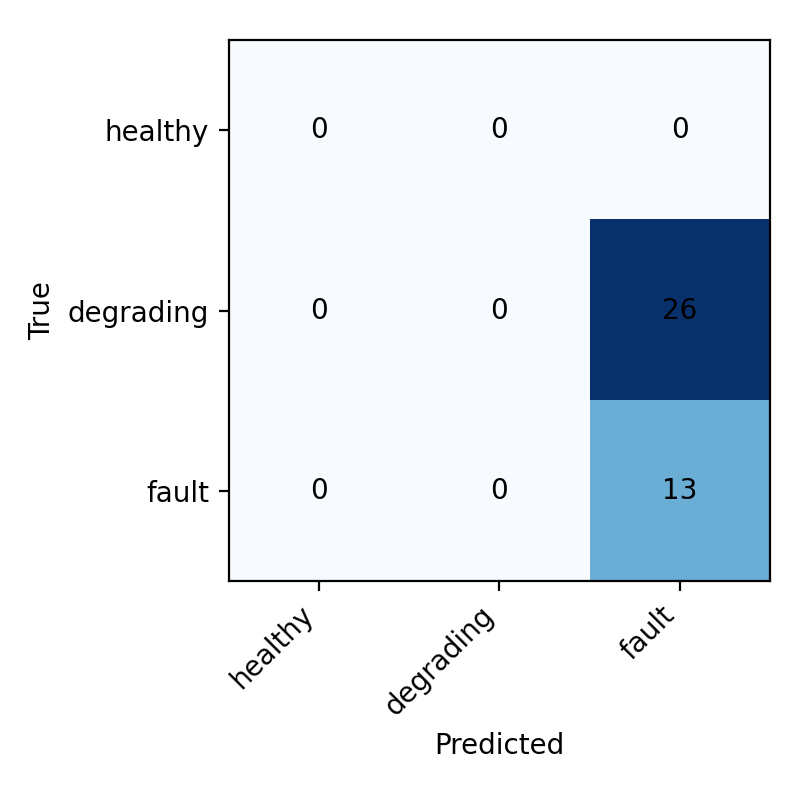
\includegraphics[width=\linewidth]{figures/ablation/temporal_scratch_confusion.png}
    \caption{From scratch (same late coverage).}
  \end{subfigure}
  \caption{Ablation on initialization: two-phase vs. from scratch under temporal evaluation.}
  \label{fig:abl_init}
\end{figure}

\paragraph{Temporal test slice.}
We further vary the temporal test slice to examine protocol effects. A broader late slice $[70,100.1]\%$ includes early Degrading and yields lower Degrading F1 (e.g., 0.07 in our run), while a very-late slice $[90,100.1]\%$ may contain only Fault (macro metrics become less informative). Figure~\ref{fig:abl_slice} shows confusion matrices for both settings.

\begin{figure}[H]
  \centering
  \begin{subfigure}[H]{0.48\textwidth}
    \centering
    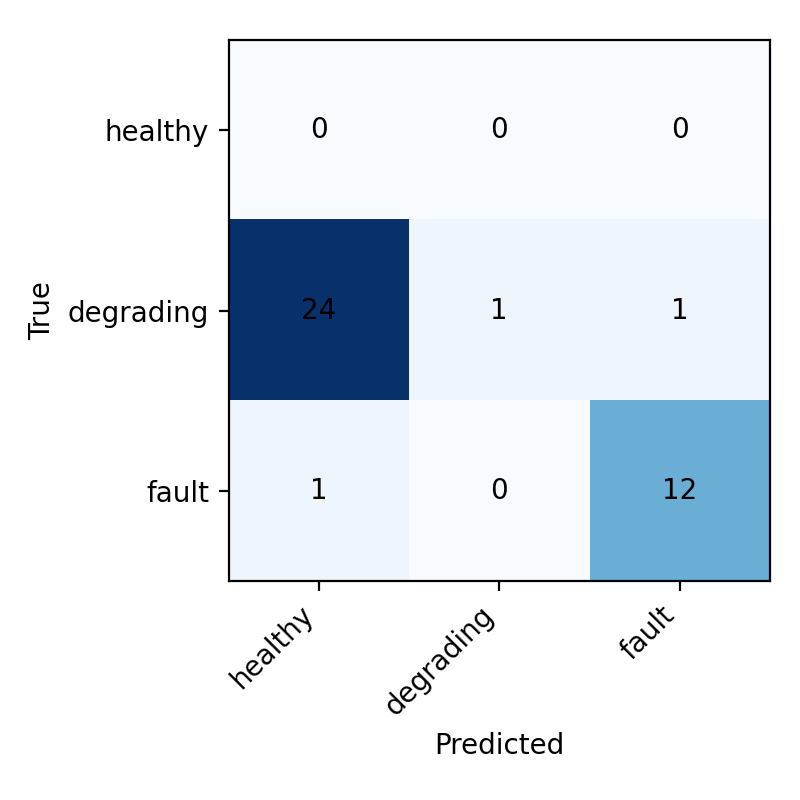
\includegraphics[width=\linewidth]{figures/ablation/temporal_broad_confusion.png}
    \caption{Broad late slice $[70,100.1]\%$ TTF.}
  \end{subfigure}
  \hfill
  \begin{subfigure}[H]{0.48\textwidth}
    \centering
    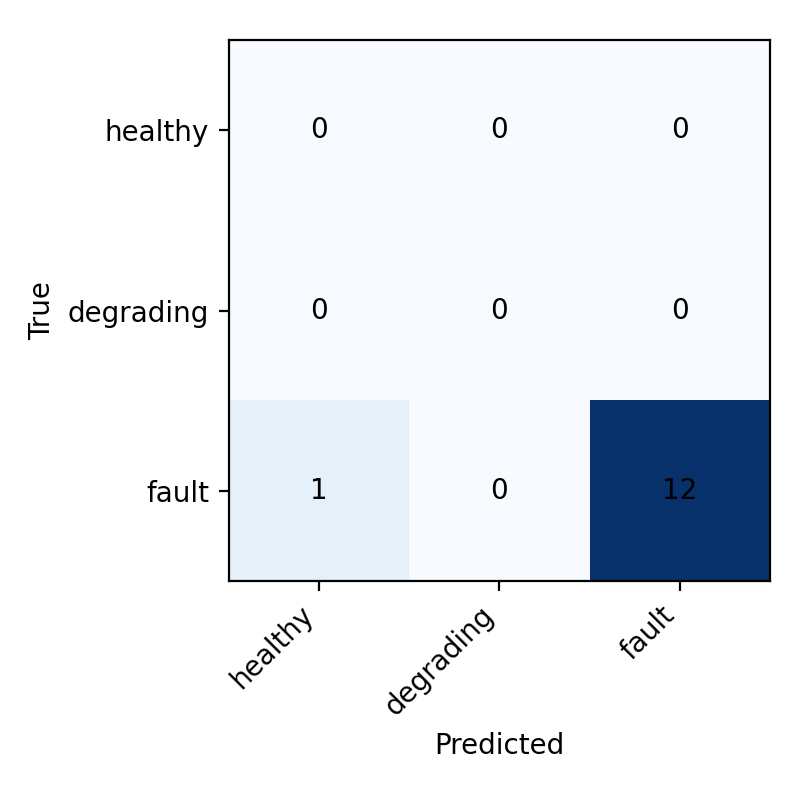
\includegraphics[width=\linewidth]{figures/ablation/temporal_late_confusion.png}
    \caption{Very-late slice $[90,100.1]\%$ TTF.}
  \end{subfigure}
  \caption{Ablation on temporal test slice selection under leakage-aware evaluation.}
\label{fig:abl_slice}
\end{figure}

\paragraph{Multi-modal fusion (vibration + temperature) vs. vibration-only.}
To assess the contribution of temperature features, we compare our multi-modal model against a vibration-only variant where the temperature branch is disabled (same training protocols; stratified pre-training followed by temporal fine-tuning). We report file-wise metrics on the late-life temporal slice (present-labels). Table~\ref{tab:mm_vs_vib} summarizes Macro-F1 and Degrading/Fault F1. In our runs, adding the 6-D temperature descriptor improves Degrading recognition while keeping Fault performance high.

\begin{table}[H]
  \centering
  \begin{tabular}{lccc}
    \hline
    Model & Macro-F1 (present) & F1 Degrading & F1 Fault \\
    \hline
    Vibration-only & 0.2593 & 0.5185 & 0.0000 \\
    Multi-modal (vib+temp) & 0.9467 & 0.9333 & 0.9600 \\
    \hline
  \end{tabular}
  \caption{Ablation: multi-modal fusion vs. vibration-only on the late-life temporal slice $[85,100.1]\%$ TTF (present-labels). Metrics are computed over present classes (Healthy absent).}
  \label{tab:mm_vs_vib}
\end{table}

\begin{figure}[H]
  \centering
  \begin{subfigure}[htbp]{0.48\textwidth}
    \centering
    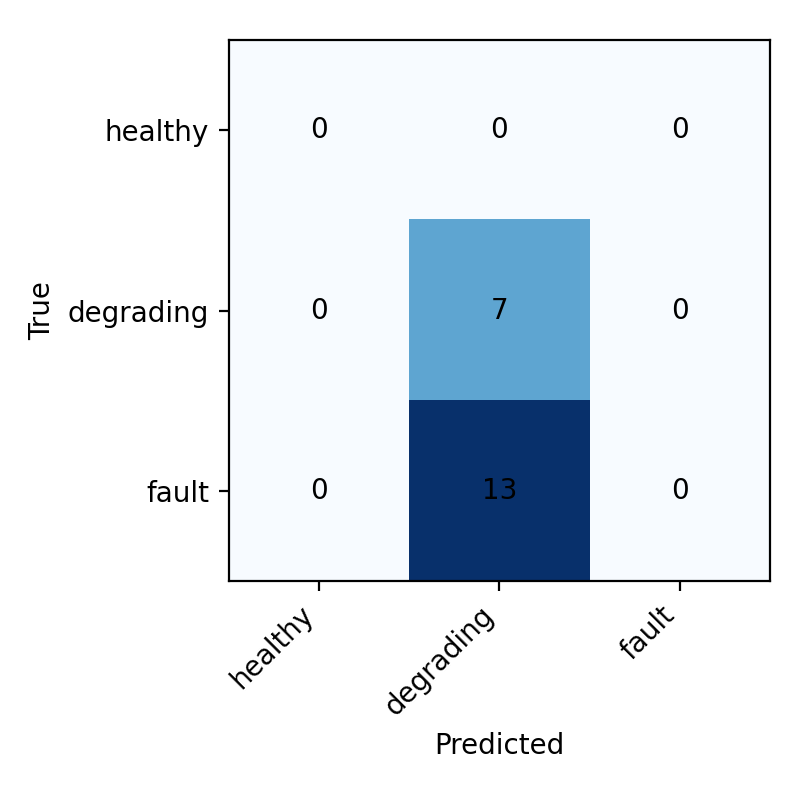
\includegraphics[width=\linewidth]{figures/ablation/vib_only_85100_confusion.png}
    \caption{Vibration-only (late-life $[85,100.1]\%$).}
  \end{subfigure}
  \hfill
  \begin{subfigure}[htbp]{0.48\textwidth}
    \centering
    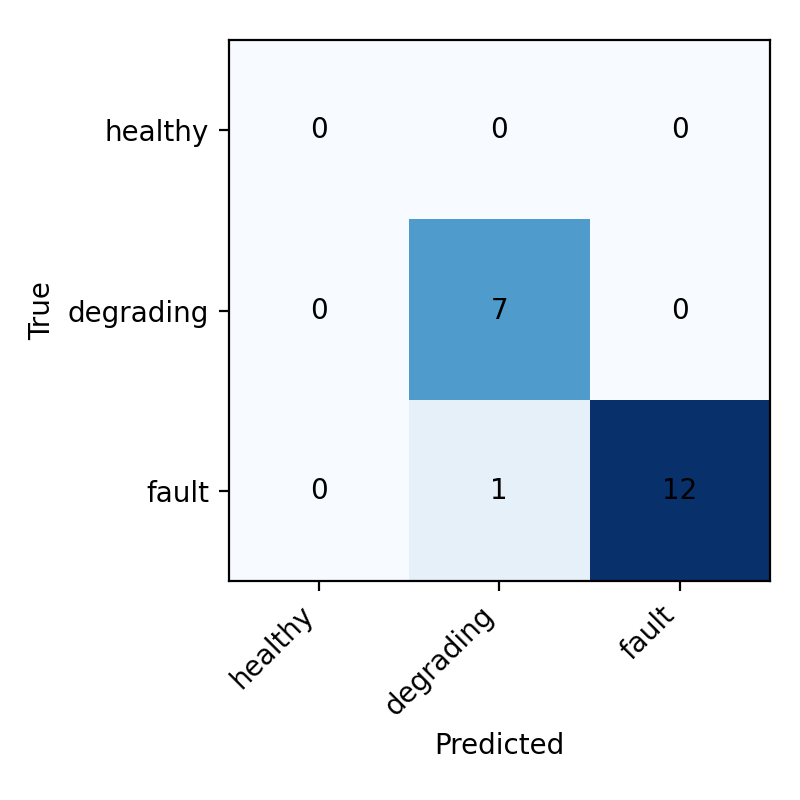
\includegraphics[width=\linewidth]{figures/ablation/multi_modal_85100_confusion.png}
    \caption{Multi-modal (late-life $[85,100.1]\%$).}
  \end{subfigure}
  \caption{Ablation (late-life $[85,100.1]\%$): confusion matrices for vibration-only vs. multi-modal on the same temporal slice (metrics computed over present classes).}
  \label{fig:mm_late_pair}
\end{figure}


\paragraph{Broad late slice $[70,100.1]\%$: multi-modal vs. vibration-only.}
To complete the comparison, we also report present-label metrics on the broader late slice. Here, the vibration-only model emphasizes Degrading (F1 $\approx$ 0.8000) but fails to recognize Fault (F1 $\approx$ 0.0000), while the multi-modal model captures Fault well (F1 $\approx$ 0.9231) but struggles with early Degrading (F1 $\approx$ 0.0741). Table~\ref{tab:mm_vs_vib_broad} summarizes these trends.

\begin{table}[htbp]
  \centering
  \begin{tabular}{lccc}
    \hline
    Model & Macro-F1 (present) & F1 Degrading & F1 Fault \\
    \hline
    Vibration-only & 0.4000 & 0.8000 & 0.0000 \\
    Multi-modal (vib+temp) & 0.3324 & 0.0741 & 0.9231 \\
    \hline
  \end{tabular}
  \caption{Broad late slice $[70,100.1]\%$ TTF (present-labels): vibration-only vs. multi-modal. Metrics are computed over present classes (Healthy absent).}
  \label{tab:mm_vs_vib_broad}
\end{table}

\begin{figure}[H]
  \centering
  \begin{subfigure}[htbp]{0.48\textwidth}
    \centering
    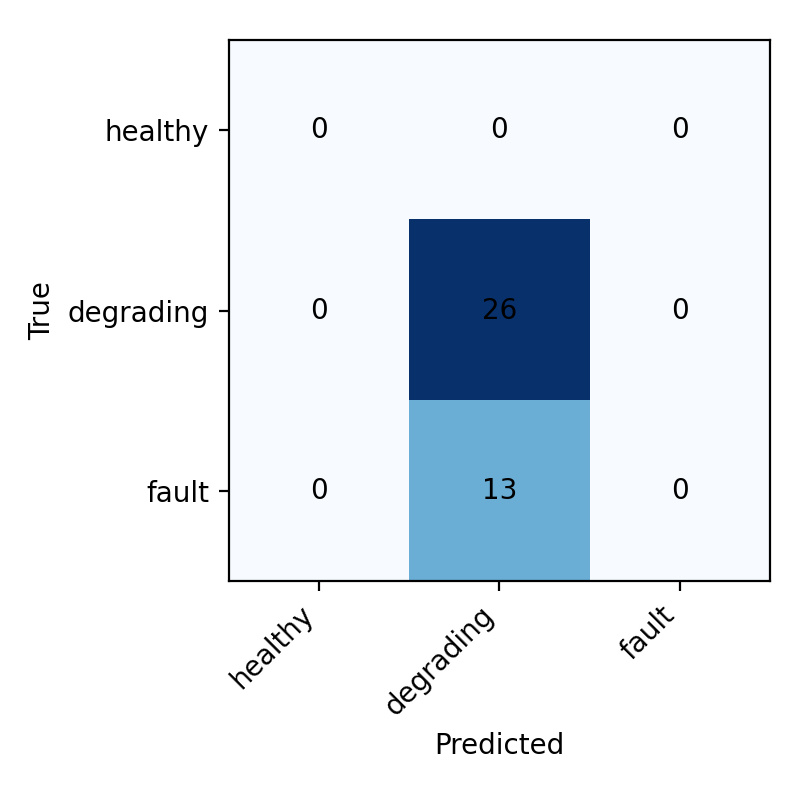
\includegraphics[width=\linewidth]{figures/ablation/vib_only_broad_confusion.png}
    \caption{Vibration-only (broad slice).}
  \end{subfigure}
  \hfill
  \begin{subfigure}[htbp]{0.48\textwidth}
    \centering
    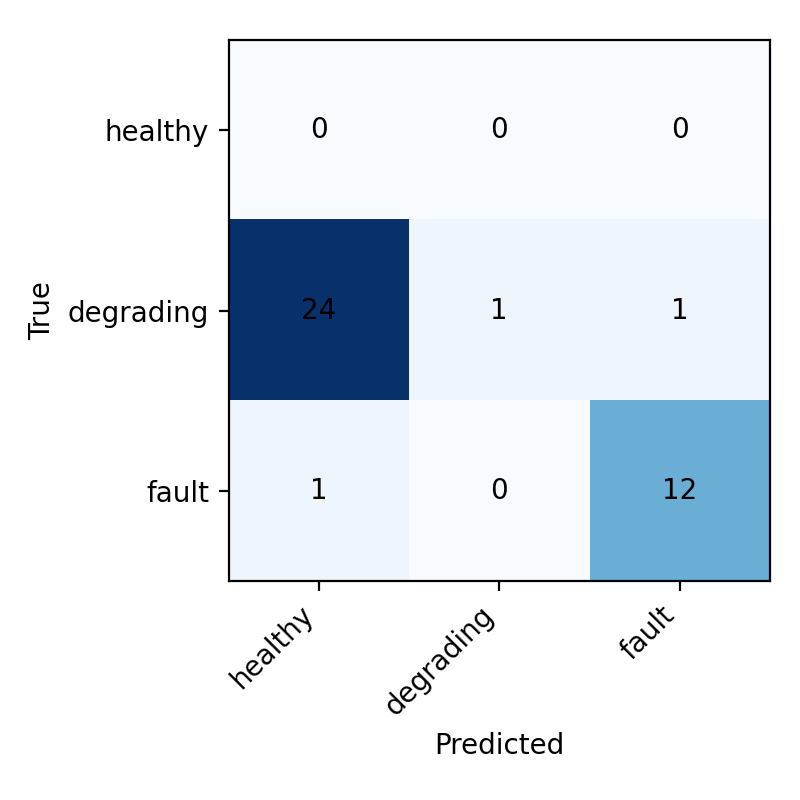
\includegraphics[width=\linewidth]{figures/ablation/multi_modal_broad_confusion.png}
    \caption{Multi-modal (broad slice).}
  \end{subfigure}
  \caption{Confusion matrices on the broad late slice $[70,100.1]\%$ for vibration-only vs. multi-modal.}
  \label{fig:mm_broad_pair}
\end{figure}


\section{Discussion and Threats to Validity}
\label{sec:discussion}

\subsection{Discussion}
Our results reinforce two practical observations for run-to-failure bearing monitoring. First, the \textit{Fault} stage is comparatively easier to separate, as late-life vibration signatures often exhibit clear and consistent spectral patterns. In contrast, the \textit{Degrading} stage is intrinsically ambiguous: it represents a transition region where signal changes can be subtle, intermittent, and partially overlapping with Healthy behavior. This is reflected by lower Degrading performance in the stratified 3-class setting and by the confusion observed when evaluation slices include earlier portions of the mid-life region.

Second, the evaluation protocol substantially affects the perceived performance. File-wise stratified splitting is useful for rapid iteration and model selection during development, but it can still overestimate deployment performance when overlapped windows introduce strong temporal correlation. The leakage-aware temporal protocol aligned with the TTF axis provides a more deployment-oriented assessment by enforcing that training data precede validation/testing along the lifetime timeline. Under late-life temporal testing, where only Degrading and Fault are present, the model maintains strong discrimination, suggesting that the learned time--frequency representation transfers from early-life training to later-life conditions when leakage is controlled.

Finally, the multi-modal design provides a simple trade-off between robustness and efficiency. Temperature descriptors add negligible computational overhead relative to the CNN encoder while offering complementary evidence about thermal trends. However, the current 6-D temperature summary is intentionally minimal; richer temporal modeling of temperature (or longer context windows) may further improve sensitivity near the Healthy--Degrading boundary.

\paragraph{What temperature adds.} On the late-life slice $[85,100.1]\%$ TTF, the vibration-only model under-performs (present-label Macro-F1 $\approx$ 0.26) compared with the multi-modal model (Macro-F1 $\approx$ 0.95), primarily due to \emph{Fault} recognition (F1 $\approx$ 0.00 vs. $\approx$ 0.96). This suggests that temperature provides complementary cues about cumulative friction/thermal load that strengthen late-life discrimination when vibration alone is ambiguous or dominated by non-stationary patterns. On the broader late slice $[70,100.1]\%$, we observe a trade-off: vibration-only emphasizes Degrading (F1 $\approx$ 0.80) while multi-modal captures Fault (F1 $\approx$ 0.92), indicating sensor complementarity across sub-regions of the lifecycle.

\subsection{Threats to validity}
\paragraph{Limited run coverage (external validity).}
Our experiments are conducted on a single run (RUNS=1) with 129 files, which limits conclusions about generalization across bearings, loads, and operating conditions. A broader evaluation with multiple runs and bearing-wise splits is needed to quantify cross-unit robustness and to assess domain shift.

\paragraph{Stage definitions based on TTF thresholds (construct validity).}
We define health stages using fixed TTF thresholds ($\tau_1=0.60$, $\tau_2=0.90$). While practical for structuring a run-to-failure timeline, these thresholds may not perfectly align with the true physical onset of degradation, and the transition region can be inherently fuzzy. Future work could refine labels using additional degradation indicators (e.g., envelope features, kurtosis trends, or expert annotations) and evaluate sensitivity to threshold choices.

\paragraph{Temporal correlation from overlapped windowing (internal validity).}
Window overlap (50\%) increases the number of training instances but also raises the risk of temporal leakage if splits are performed at the window level. We mitigate this with a TTF-aligned temporal protocol; nonetheless, residual correlation may remain near split boundaries. Introducing a temporal ``gap'' between train/val/test segments or using non-overlapping evaluation windows are potential safeguards.

\paragraph{Class presence in temporal slices (metric interpretation).}
In late-life temporal testing ([70,100.1]\% TTF), Healthy samples may be absent. Reporting macro metrics over all three classes would be misleading due to zero-support classes. We therefore report performance over the \emph{present classes} for the temporal slice and explicitly state class coverage when interpreting results.

\paragraph{Synchronous sampling assumption (deployment validity).}
The current pipeline assumes vibration and temperature are synchronously sampled and windowed using identical indices. If temperature is sampled at a different rate in real deployments, explicit resampling and timestamp alignment will be required before feature extraction. This engineering constraint may affect end-to-end performance and should be validated in future deployments.

\section{Conclusion and Future Work}
\label{sec:conclusion}

This paper investigated three-stage bearing health classification (Healthy, Degrading, Fault) in a run-to-failure setting using a lightweight multi-modal model that fuses STFT-based vibration representations with compact temperature trend descriptors. Beyond a stratified development evaluation, we emphasized a \textbf{leakage-aware temporal protocol} aligned with the TTF timeline and a two-phase workflow (stratified training $\rightarrow$ temporal fine-tuning) to better approximate deployment conditions. Experimental results show strong late-life discrimination between Degrading and Fault under temporal evaluation, while the Healthy--Degrading boundary remains the most challenging region when broader mid-life coverage is included. Our choice of TTF thresholds (60\%/90\%) is motivated by empirical observation on this run; we view the present study as a \emph{proof of concept} and plan to examine threshold sensitivity and validate on additional datasets (e.g., CWRU, Paderborn) to strengthen generality.

\textbf{Future work} will focus on: (i) extending evaluation to multiple runs/bearings and external datasets (e.g., CWRU, Paderborn), and performing bearing-wise splits to quantify generalization under domain shift; (ii) improving supervision in the transition region via refined degradation indicators or expert-informed labeling beyond fixed TTF thresholds; (iii) incorporating longer temporal context with sequence-aware models to better capture gradual degradation dynamics; and (iv) exploring calibration and uncertainty estimation to support reliable early-warning decisions in practical CBM deployments.

\section*{Code and Data Availability}
The dataset used in this study is publicly available \cite{jung2024dib_rtf,jung2024mendeley_rtf}. Our code and configuration files for reproducing the preprocessing, splits, and evaluation will be released upon acceptance. Our implementation adapts components from an upstream open-source repository~\cite{mdzalfirdausi_paderborn_repo} and is customized for: (i) a TTF-aligned temporal split to avoid leakage, (ii) per-window and per-frequency spectrogram normalization, (iii) 6-D temperature feature fusion with a lightweight head, and (iv) file-wise aggregation via mean pre-softmax logits.
\bibliographystyle{IEEEtran}
\bibliography{refs}

\end{document}
